\documentclass[12pt]{article}
\usepackage{geometry}
\geometry{letterpaper}
\usepackage{amssymb}
\usepackage{amsmath}
\usepackage{listings}
\usepackage{fancyhdr}
\usepackage{url}
\newcounter{ProblemNum}
\newcounter{SubProblemNum}[ProblemNum]
\newcommand{\divides}{\bigm|}
\renewcommand{\theProblemNum}{\arabic{ProblemNum}}
\renewcommand{\theSubProblemNum}{\alph{SubProblemNum}}
\newcommand*{\anyproblem}[1]{\newpage\subsection*{#1}}
\newcommand*{\problem}[1]{\stepcounter{ProblemNum} %
\anyproblem{Problem \theProblemNum. \; #1}}
\newcommand*{\soln}[1]{\subsubsection*{#1}}
\newcommand*{\solution}{\soln{Solution}}
\renewcommand*{\part}{\stepcounter{SubProblemNum} %
\soln{Part (\theSubProblemNum)}}
\usepackage{graphicx}
\graphicspath{ {./images/} }
\usepackage{float}
\usepackage{pythonhighlight}
% Document metadata
% Document starts here
\begin{document}
\begin{center}
\begin{Large}
  \textbf{CSC413 Assignment 1}\\
\end{Large}
\begin{large}
	Ming Gong   1004709130\\
	Hongyu Chen 1005398197
\end{large}
\end{center}
%\vspace{-.5in}

\begin{python}
import pandas
import numpy as np
import matplotlib.pyplot as plt

import torch
import torch.nn as nn
import torch.optim as optim
\end{python}

Question 1:Data\\
\begin{python}
from google.colab import drive
drive.mount('/content/gdrive')
file_path = '/content/gdrive/My Drive/CSC413/A1/raw_sentences.txt'

!ls /content/gdrive/My\ Drive/
!mkdir /content/gdrive/My\ Drive/CSC413

sentences = []
for line in open(file_path):
    words = line.split()
    sentence = [word.lower() for word in words]
    sentences.append(sentence)

vocab = set([w for s in sentences for w in s])
print(len(sentences)) # 97162
print(len(vocab)) # 250

test, valid, train = sentences[:10000], sentences[10000:20000], sentences[20000:]
\end{python}

Part (a) \\
Display 10 sentences in the training set. Explain how punctuations are treated in our word representation, and how words with apostrophes are represented.\\
\begin{python}
for i in range(10):
  print(train[i])
  
output:
['last', 'night', ',', 'he', 'said', ',', 'did', 'it', 'for', 'me', '.']
['on', 'what', 'can', 'i', 'do', '?']
['now', 'where', 'does', 'it', 'go', '?']
['what', 'did', 'the', 'court', 'do', '?']
['but', 'at', 'the', 'same', 'time', ',', 'we', 'have', 'a', 'long', 'way', 'to', 'go', '.']
['that', 'was', 'the', 'only', 'way', '.']
['this', 'team', 'will', 'be', 'back', '.']
['so', 'that', 'is', 'what', 'i', 'do', '.']
['we', 'have', 'a', 'right', 'to', 'know', '.']
['now', 'they', 'are', 'three', '.']
\end{python}
Punctuations are treated as a single words in our word representation except for apostrophes.  Apostrophe will combine with the rest of the word/letters after itself and the whole combination will be inside a double quotation mark in the display.\\

Part (b)\\
What are the 10 most common words in the vocabulary? How often does each of these words appear in the training sentences? Express the second quantity a percentage (i.e. number of occurrences of the word / total number of words in the training set).\\
These are good quantities to compute, because one of the first things that most machine learning model will learn is to predict the most common class. Getting a sense of the distribution of our data will help you understand our model's behaviour.\\
You might find Python's collections.Counter class helpful.\\
\begin{python}
from collections import Counter
count = Counter([item for sublist in train for item in sublist])
common_word = sorted(count, key=count.get,reverse=True)
times = sorted(count.values(),reverse=True)
total = sum(count.values())
print("10 most common words in the vocabulary : ", common_word[:10])
print("total time each of these words appear in the training sentences : ",times[:10])
print("Precentage of these words appear in the training sentences : ", [x / total for x in times[:10]])
\end{python}
10 most common words in the vocabulary :  ['.', 'it', ',', 'i', 'do', 'to', 'nt', '?', 'the', "'s"]\\
total time each of these words appear in the training sentences :  [64297, 23118, 19537, 17684, 16181, 15490, 13009, 12881, 12583, 12552]\\
Precentage of these words appear in the training sentences :  [0.10695720015237538, 0.038456484021379134, 0.032499538382458865, 0.029417097648328946, 0.026916877236349845, 0.02576740797176065, 0.021640297631028683, 0.021427371341784955, 0.020931652324639397, 0.020880084238963183]\\

Part (c)\\
Complete the helper functions $convert\_words\_to\_indices$ and $generate\_4grams$, so that the function $process\_data$will take a list of sentences (i.e. list of list of words), and generate an  $Nx4$ numpy matrix containing indices of 4 words that appear next to each other. You can use the constants vocab, $vocab\_itos$, and $vocab\_stoi$ in your code.\\
\begin{python}
# A list of all the words in the data set. We will assign a unique 
# identifier for each of these words.
vocab = sorted(list(set([w for s in train for w in s])))
# A mapping of index => word (string)
vocab_itos = dict(enumerate(vocab))
# A mapping of word => its index
vocab_stoi = {word:index for index, word in vocab_itos.items()}

def convert_words_to_indices(sents):
    """
    This function takes a list of sentences (list of list of words)
    and returns a new list with the same structure, but where each word
    is replaced by its index in `vocab_stoi`.

    Example:
    >>> convert_words_to_indices([['one', 'in', 'five', 'are', 'over', 'here'],
                                  ['other', 'one', 'since', 'yesterday'],
                                  ['you']])
    [[148, 98, 70, 23, 154, 89], [151, 148, 181, 246], [248]]
    """

    indices = []
    for sentence in sents:
      sen_index = []
      for letter in sentence:
        sen_index.append(vocab_stoi[letter])
      indices.append(sen_index)
    return indices


def generate_4grams(seqs):
    """
    This function takes a list of sentences (list of lists) and returns
    a new list containing the 4-grams (four consequentively occuring words)
    that appear in the sentences. Note that a unique 4-gram can appear multiple
    times, one per each time that the 4-gram appears in the data parameter `seqs`.

    Example:

    >>> generate_4grams([[148, 98, 70, 23, 154, 89], [151, 148, 181, 246], [248]])
    [[148, 98, 70, 23], [98, 70, 23, 154], [70, 23, 154, 89], [151, 148, 181, 246]]
    >>> generate_4grams([[1, 1, 1, 1, 1]])
    [[1, 1, 1, 1], [1, 1, 1, 1]]
    """
    grams4 = []
    for sentence in seqs:
      while len(sentence) >= 4:
        grams4.append(sentence[0:4])
        sentence.pop(0)
    return grams4


def process_data(sents):
    """
    This function takes a list of sentences (list of lists), and generates an
    numpy matrix with shape [N, 4] containing indices of words in 4-grams.
    """
    indices = convert_words_to_indices(sents)
    fourgrams = generate_4grams(indices)
    return np.array(fourgrams)

train4grams = process_data(train)
valid4grams = process_data(valid)
test4grams = process_data(test)
\end{python}

Question 2. MLP Math\\

Part(a)\\
What is the shape of the input vector  x? What is the shape of the output vector  y? Let  k  represent the size of the hidden layer. What are the dimension of  W(1)  and  W(2) ?\\
The shape of x is (750, 1). The shape of y is (250, 1). The dimension of $W^{(1)}$ is (k, 750) and the dimension of $W^{(2)}$ is (250, k).\\

Part(b)\\
Draw a computation graph for  y. Your graph should include the quantities  W(1) ,  W(2) ,  b(1) ,  b(2) ,  x ,  m,  h,  z  and  y.\\
\begin{figure}[H]
    \centering
    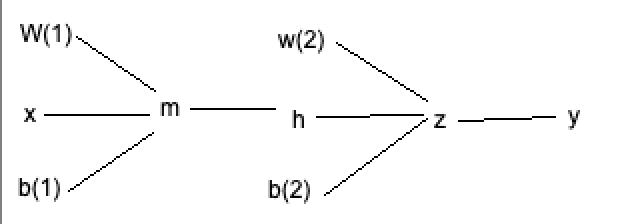
\includegraphics[width=100mm,scale=1]{2}\

\end{figure}


Part(c)\\
Derive the gradient descent update rule for  W(2) . You should begin by deriving the update rule for  $W_{ij}^{(2)} $, and then vectorize your answer. Assume that we will use the softmax activation and cross-entropy loss.\\
\begin{figure}[H]
    \centering
    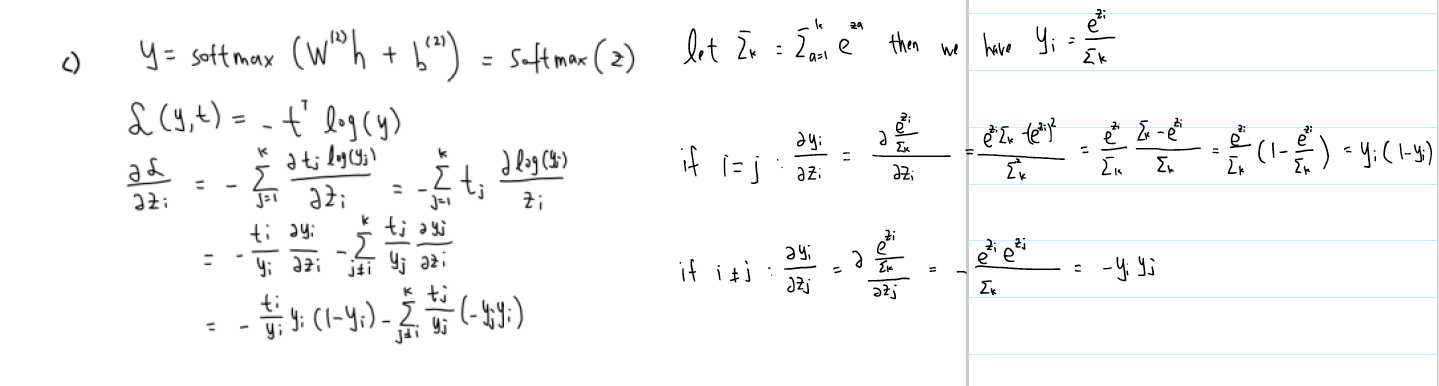
\includegraphics[width=170mm,scale=2]{2c1}\
    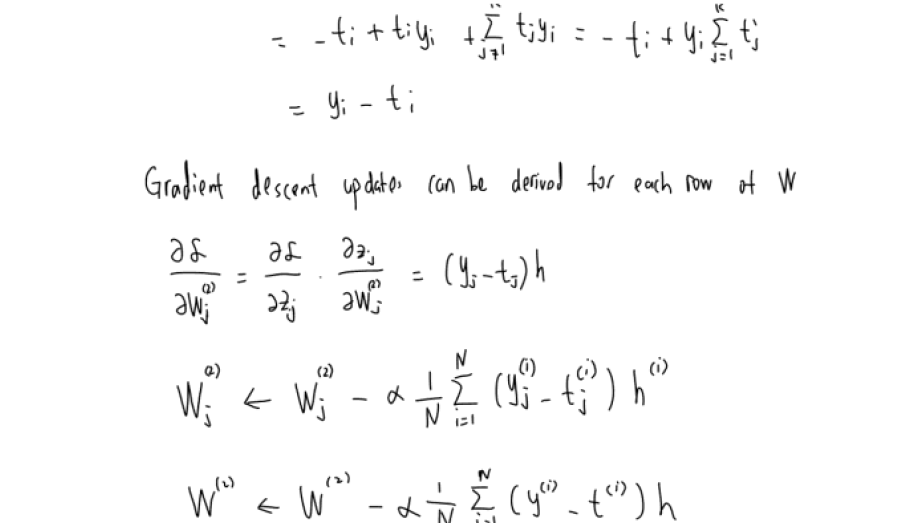
\includegraphics[width=170mm,scale=1.5]{2c2}\

\end{figure}

Part(d)\\
What would be the update rule for  $W^{(2)}_{ij}$ , if we use the square loss  $\mathcal{L}_{SE}(y, t) = \frac{1}{2}(y-t)^2$  ?
Show that we will not get good gradient signal to update  $W^{(2)}_{ij}$  if we use this square loss.\\
\begin{figure}[H]
    \centering
    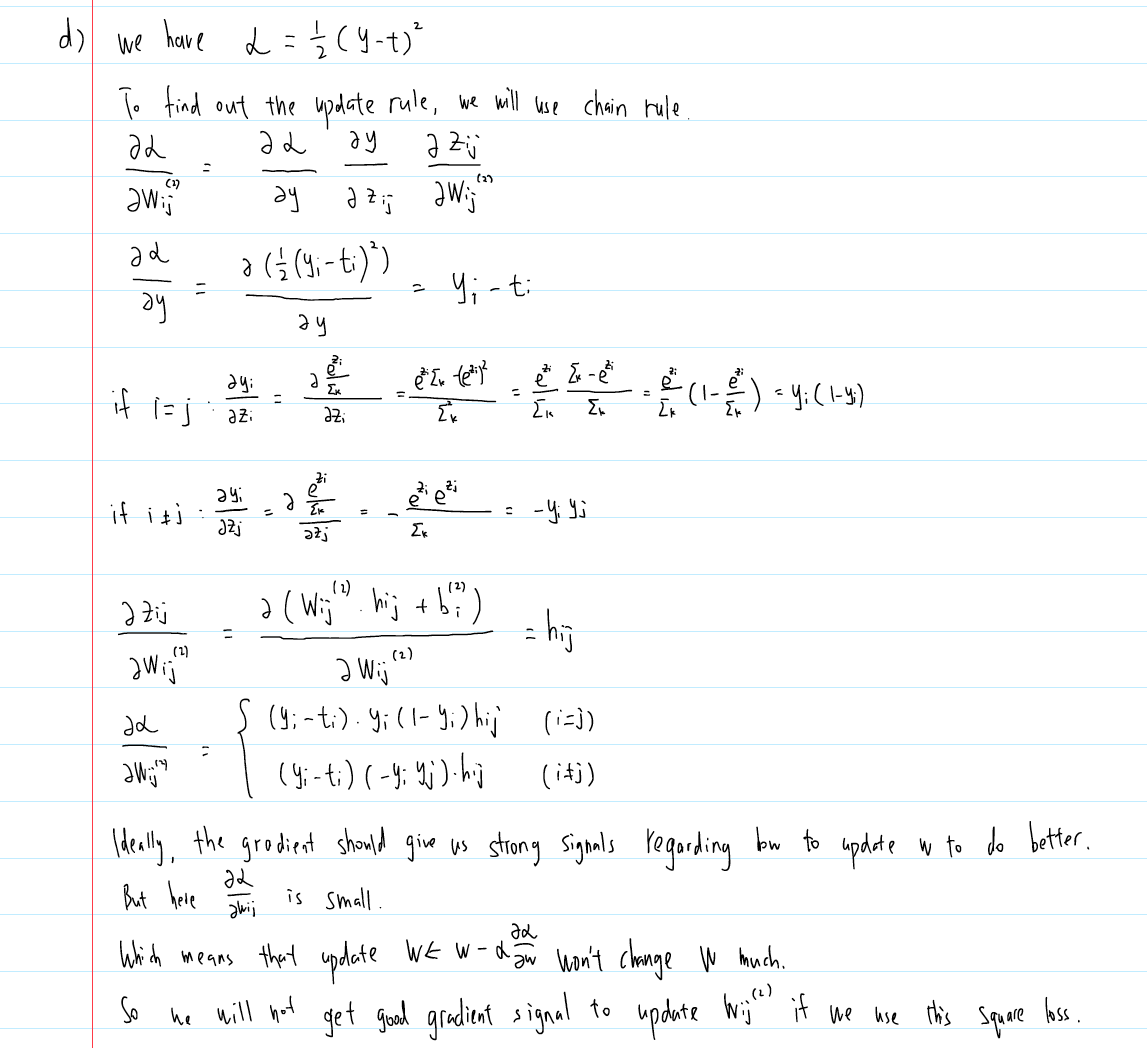
\includegraphics[width=170mm,scale=2]{2d}\

\end{figure}

Part(e)\\
$\sigma^{'} (z)  = -(1+e^{-z})^{-2}(-e^{-z}) = \frac{1}{1+e^{-z}}\frac{e^{-z}}{1+e^{-z}} = \frac{1}{1+e^{-z}}\frac{1+e^{-z}-1}{1+e^{-z}}
= \frac{1}{1+e^{-z}}(\frac{1+e^{-z}}{1+e^{-z}} - \frac{1}{1+e^{-z}}) = \frac{1}{1+e^{-z}}(1-\frac{1}{1+e^{-z}}) = \sigma(z)(1-\sigma(z))$\\
\begin{figure}[H]
    \centering
    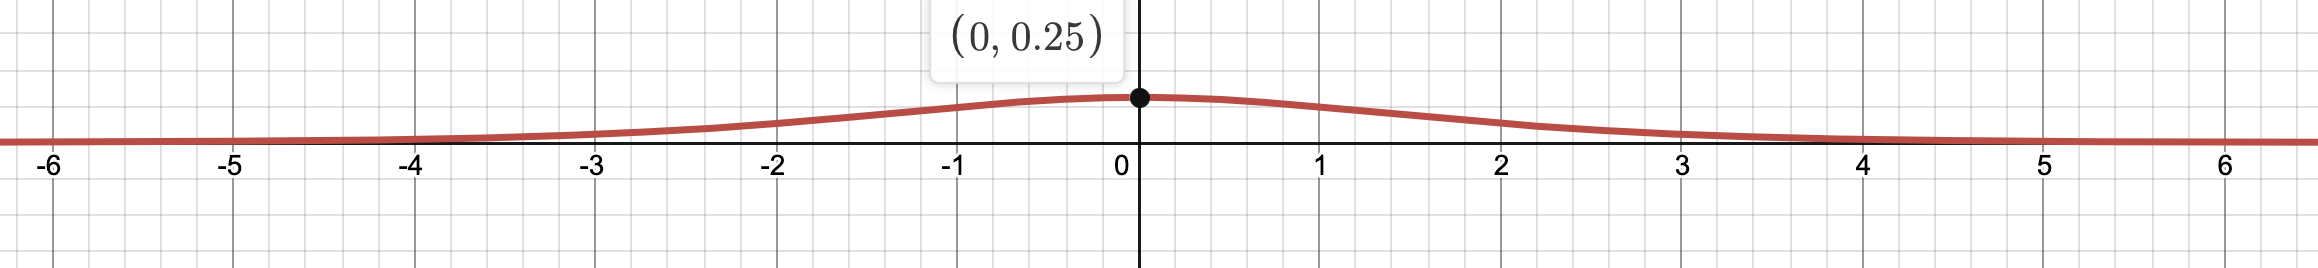
\includegraphics[width=100mm,scale=0.5]{e}\
    \caption{Plot for $\sigma^{'}(z)$}
\end{figure}
Max: let $\sigma^{''}(z) = -\frac{e^z-1)e^z}{(e^z+1)^3} = 0$\\
$-(e^z-1)e^z = 0 \rightarrow e^z-1 = 0 \rightarrow e^{z} = 1 \rightarrow z = 0$\\ 
When z = 0, $\sigma^{'}(0) = 0.25 = \frac{1}{4}$. So the maximum is (0, 0.25) and $\sigma^{'}(z)$ must be positive since both $e^{-z} $ and $(e^{-z}+1) $ are positive. \\
$\frac{\partial h_1 }{\partial x} = \frac{\partial h_1 }{\partial z}\frac{\partial z}{\partial x} = \sigma^{'}(z)*w_1$. Depends on the plot of $\sigma^{'}(z)$ the maximum point is 1/4 and  $\sigma^{'}(z)$ is positive. so $|\frac{\partial h_1 }{\partial x}| \leq \frac{1}{4}|w_1|$ holds.\\

Part(f)\\
$|\frac{\partial h_N }{\partial x} |= |\frac{\partial h_N }{\partial h_{N-1}}||\frac{\partial h_{N-1} }{\partial h_{N-2}}| .... |\frac{\partial h_1 }{\partial x}| \leq  \frac{1}{4}|w_N|\frac{1}{4}|w_{N-1}| .... \frac{1}{4}|w_1| = \frac{1}{4^{N}}|w_N| ....|w_1|$\\
The problem is when N is very large, $|\frac{\partial h_N }{\partial x} $ will become extremely small. Since it's smaller than $\frac{1}{4^{N}}|w_N| ....|w_1|$ and $\frac{1}{4^{N}}$ will be surely very small when N is big. And this means that x's value will not effect $h_N$ a lot. The Nth layer will try to update its
weight mostly based on its previous layer's updated weight. More closer to the last layer,
the value of x will be less important. In this case, for many of the layers close to the Nth
layer, it will only take few information from the input x. It shows that more layers will not
help at all and it will even make the learning speed slower and cause problems. On the
other hand, if we have many layers and we multiply these gradients together, it's possible
that the product of many small values (less than one) will become zero very quickly
(because "1/a large number" will be treated as 0 if the number is large enough) since the
derivative of the sigmoid function is always smaller than 1. For deep learning, more layers
will always improve the learning experience, but if we use sigmoid activation function,
more layers means problems. That's why sigmoid activation function would be a problem
with this result.\\

Part(g)\\
Would we have the same issue as in part(f) we we replaced the sigmoid activation with ReLU activations? Why or why not?\\
No, we will not have the same issue as in part f if we replaced the sigmoid activation with
ReLu activation. ReLu activation function reduced likelihood of the gradient to vanish. For
the gradient of sigmoid activation function, it will get smaller and smaller as the absolute
value of the input x increases. And as we saw in the previous questions, the derivative of
the sigmoid function is always smaller than $\frac{1}{4}$. In part (e) we just proved that the
maximum is (0,$\frac{1}{4}$). It means that the sigmoid activation function learns slow. But the
constant gradient of ReLus will have a faster learning. The gradient of the ReLu activation
function is either 0 (if <0) or 1 (if >0). This means the number of the layers will not cause
any problems. The gradients will never vanish.

Question 3. Weight Sharing - Math\\
Part(a) \\
\begin{figure}[H]
    \centering
    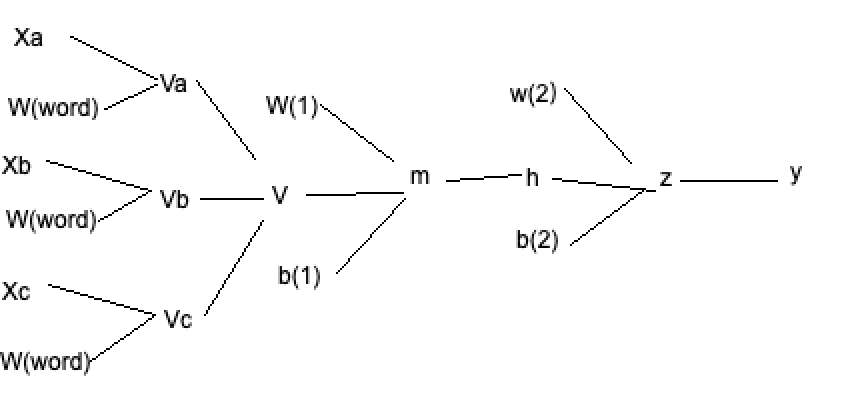
\includegraphics[width=100mm,scale=1]{3}\

\end{figure}

Part(b)\\
$\frac{\partial y}{\partial W^{(word)}} =\frac{\partial y}{\partial z}\frac{\partial z}{\partial W^{(word)}}= \frac{\partial y}{\partial z}\frac{\partial z}{\partial h}\frac{\partial h}{\partial W^{(word)}}\\
 = \frac{\partial y}{\partial z}\frac{\partial z}{\partial h}\frac{\partial h}{\partial m}\frac{\partial m}{\partial W^{(word)}} 
= \frac{\partial y}{\partial z}\frac{\partial z}{\partial h}\frac{\partial h}{\partial m}\frac{\partial m}{\partial v} \frac{\partial v}{\partial W^{(word)}}\\ =
 \frac{\partial y}{\partial z} \frac{\partial z}{\partial h} \frac{\partial h}{\partial m}\frac{\partial m}{\partial v} (\frac{\partial v}{\partial v_a}\frac{\partial v_a}{\partial W^{(word)}} + \frac{\partial v}{\partial v_b}\frac{\partial v_b}{\partial W^{(word)}} +\frac{\partial v}{\partial v_c}\frac{\partial v_c}{\partial W^{(word)}})$\\

Question 4. Numpy\\
\begin{python}
def make_onehot(indicies, total=250):
    """
    Convert indicies into one-hot vectors by
        1. Creating an identity matrix of shape [total, total]
        2. Indexing the appropriate columns of that identity matrix
    """
    I = np.eye(total)
    return I[indicies]

def softmax(x):
    """
    Compute the softmax of vector x, or row-wise for a matrix x.
    We subtract x.max(axis=0) from each row for numerical stability.
    """
    x = x.T
    exps = np.exp(x - x.max(axis=0))
    probs = exps / np.sum(exps, axis=0)
    return probs.T

def get_batch(data, range_min, range_max, onehot=True):
    """
    Convert one batch of data in the form of 4-grams into input and output
    data and return the training data (xs, ts) where:
     - `xs` is an numpy array of one-hot vectors of shape [batch_size, 3, 250]
     - `ts` is either
            - a numpy array of shape [batch_size, 250] if onehot is True,
            - a numpy array of shape [batch_size] containing indicies otherwise

    Preconditions:
     - `data` is a numpy array of shape [N, 4] produced by a call
        to `process_data`
     - range_max > range_min
    """
    xs = data[range_min:range_max, :3]
    xs = make_onehot(xs)
    ts = data[range_min:range_max, 3]
    if onehot:
        ts = make_onehot(ts).reshape(-1, 250)
    return xs, ts

def estimate_accuracy(model, data, batch_size=5000, max_N=100000):
    """
    Estimate the accuracy of the model on the data. To reduce
    computation time, use at most `max_N` elements of `data` to
    produce the estimate.
    """
    correct = 0
    N = 0
    for i in range(0, data.shape[0], batch_size):
        xs, ts = get_batch(data, i, i + batch_size, onehot=False)
        z = model(xs)
        pred = np.argmax(z, axis=1)
        correct += np.sum(ts == pred)
        N += ts.shape[0]

        if N > max_N:
            break
    return correct / N
\end{python}

Part(a)\\
\begin{python}
class NumpyWordEmbModel(object):
    def __init__(self, vocab_size=250, emb_size=100, num_hidden=100):
        """
        Initialize the weights and biases to zero. Update this method
        so that weights and baises have the correct shape.
        """
        self.vocab_size = vocab_size
        self.emb_size = emb_size
        self.num_hidden = num_hidden
        self.emb_weights = np.zeros((self.emb_size, self.vocab_size)) 
        self.weights1 = np.zeros((self.num_hidden, 3 * self.emb_size))  
        self.bias1 = np.zeros(self.num_hidden)            
        self.weights2 = np.zeros((self.vocab_size, self.num_hidden))   
        self.bias2 = np.zeros(self.vocab_size)            
        self.cleanup()

    def initializeParams(self):
        """
        Randomly initialize the weights and biases of this two-layer MLP.
        The randomization is necessary so that each weight is updated to
        a different value.

        You do not need to change this method.
        """
        self.emb_weights = np.random.normal(0, 2/self.emb_size, self.emb_weights.shape)
        self.weights1 = np.random.normal(0, 2/self.emb_size, self.weights1.shape)
        self.bias1 = np.random.normal(0, 2/self.emb_size, self.bias1.shape)
        self.weights2 = np.random.normal(0, 2/self.num_hidden, self.weights2.shape)
        self.bias2 = np.random.normal(0, 2/self.num_hidden, self.bias2.shape)

    def forward(self, inputs):
        """
        Compute the forward pass prediction for inputs.

        Note that for vectorization, `inputs` will be a rank-3 numpy array
        with shape [N, 3, vocab_size], where N is the batch size.
        The returned value will contain the predictions for the N
        data points in the batch, so the return value shape should be
        [N, something].

        You should refer to the mathematical expressions we provided in Q3
        when completing this method. However, because we are computing
        forward pass for a batch of data at a time, you may need to rearrange
        some computation (e.g. some matrix-vector multiplication will become
        matrix-matrix multiplications, and you'll need to be careful about
        arranging the dimensions of your matrices.)

        For numerical stability reasons, we will return the **logit z**
        instead of the **probability y**. The loss function assumes that 
        we return the logits from this function.

        After writing this function, you might want to check that your code
        runs before continuing, e.g. try

            xs, ts = get_batch(train4grams, 0, 8, onehot=True)
            m = NumpyWordEmbModel()
            m.forward(xs)
        """
        self.N = inputs.shape[0]
        ipt = np.split(inputs,3,axis=1)
        self.xa = ipt[0].reshape((self.N,inputs.shape[2])) 
        self.xb = ipt[1].reshape((self.N,inputs.shape[2])) 
        self.xc = ipt[2].reshape((self.N,inputs.shape[2])) 
        self.va = self.xa @ (self.emb_weights).T 
        self.vb = self.xb @ (self.emb_weights).T 
        self.vc = self.xc @ (self.emb_weights).T 
        self.v = np.concatenate([self.va,self.vb,self.vc],axis=1) 
        self.m = self.v @ (self.weights1).T + self.bias1 
        self.h = np.maximum(self.m, 0) # todo
        self.z = self.h @ (self.weights2).T + self.bias2 
        self.y = softmax(self.z)
        return self.z



    def __call__(self, inputs):
        """
        This function is here so that if you call the object like a function,
        the `backward` method will get called. For example, if we have
            m = NumpyWordEmbModel()
        Calling `m(foo)` is equivalent to calling `m.forward(foo)`.

        You do not need to change this method.
        """
        return self.forward(inputs)

    def backward(self, ts):
        """
        Compute the backward pass, given the ground-truth, one-hot targets.
        Note that `ts` needs to be a numpy array with shape [N, vocab_size].
        Complete this method. You might want to refer to your answers to Q2
        and Q3. But be careful: we are computing the backward pass for an
        entire batch of data at a time! Carefully track the dimensions of your
        quantities!

        You may assume that the forward() method has already been called, so
        you can access values like self.N, self.y, etc..

        This function needs to be called before calling the update() method.
        """
        z_bar = (self.y - ts) / self.N
        self.w2_bar = z_bar.T @ self.h 
        self.b2_bar = z_bar.T @ np.ones(self.N) 
        h_bar = z_bar @ self.weights2 
        m_bar = (self.m > 0) * h_bar 
        self.w1_bar = m_bar.T @ self.v 
        self.b1_bar = m_bar.T @ np.ones(self.N) 
        # ...
        v_bar = m_bar @ self.weights1
        v_bar0 = (v_bar[:,:self.num_hidden]).T @ self.xa
        v_bar1 = (v_bar[:,self.num_hidden:self.num_hidden*2]).T @ self.xb
        v_bar2 = (v_bar[:,self.num_hidden*2:]).T @ self.xc
        self.emb_bar = v_bar0 + v_bar1 + v_bar2

    def update(self, alpha):
        """
        Compute the gradient descent update for the parameters.
        Complete this method. Use `alpha` as the learning rate.

        You can assume that the forward() and backward() methods have already
        been called, so you can access values like self.w1_bar.
        """
        self.weights1 = self.weights1 - alpha * self.w1_bar
        self.bias1 = self.bias1 - alpha * self.b1_bar
        self.weights2 = self.weights2 - alpha * self.w2_bar
        self.bias2 = self.bias2 - alpha * self.b2_bar
        self.emb_weights = self.emb_weights - alpha * self.emb_bar

    def cleanup(self):
        """
        Erase the values of the variables that we use in our computation.
       
        You do not need to change this method.
        """
        self.N = None
        self.xa = None
        self.xb = None
        self.xc = None
        self.va = None
        self.vb = None
        self.vc = None
        self.v = None
        self.m = None
        self.h = None
        self.z = None
        self.y = None
        self.z_bar = None
        self.w2_bar = None
        self.b2_bar = None
        self.w1_bar = None
        self.b1_bar = None
        self.emb_bar = None
\end{python}
 Part(b)\\
\begin{python}
def run_gradient_descent(model,
                         train_data=train4grams,
                         validation_data=valid4grams,
                         batch_size=100,
                         learning_rate=0.1,
                         max_iters=5000):
    """
    Use gradient descent to train the numpy model on the dataset train4grams.
    """
    n = 0
    while n < max_iters:
        # shuffle the training data, and break early if we don't have
        # enough data to remaining in the batch
        np.random.shuffle(train_data)
        for i in range(0, train_data.shape[0], batch_size):
            if (i + batch_size) > train_data.shape[0]:
                break

            # get the input and targets of a minibatch
            xs, ts = get_batch(train_data, i, i + batch_size, onehot=True)

            # erase any accumulated gradients
            model.cleanup()

            # forward pass: compute prediction

            y = softmax(model.forward(xs))
            # backward pass: compute error 
            model.backward(ts)
            model.update(learning_rate)
            # increment the iteration count
            n += 1

            # compute and plot the *validation* loss and accuracy
            if (n % 100 == 0):
                train_cost = -np.sum(ts * np.log(y)) / batch_size
                train_acc = estimate_accuracy(model, train_data)
                val_acc = estimate_accuracy(model, validation_data)
                model.cleanup()
                print("Iter %d. [Val Acc %.0f%%] [Train Acc %.0f%%, Loss %f]" % (
                      n, val_acc * 100, train_acc * 100, train_cost))

        if n >= max_iters:
            return


numpy_model= NumpyWordEmbModel()
numpy_model.initializeParams()
run_gradient_descent(numpy_model)
\end{python}
\begin{python}
Iter 100. [Val Acc 17%] [Train Acc 17%, Loss 5.090020]
Iter 200. [Val Acc 17%] [Train Acc 17%, Loss 4.796250]
Iter 300. [Val Acc 17%] [Train Acc 17%, Loss 4.572593]
Iter 400. [Val Acc 17%] [Train Acc 17%, Loss 4.354664]
Iter 500. [Val Acc 17%] [Train Acc 17%, Loss 4.379154]
Iter 600. [Val Acc 17%] [Train Acc 17%, Loss 4.646561]
Iter 700. [Val Acc 17%] [Train Acc 17%, Loss 4.456584]
Iter 800. [Val Acc 17%] [Train Acc 17%, Loss 4.508409]
Iter 900. [Val Acc 17%] [Train Acc 17%, Loss 4.247037]
Iter 1000. [Val Acc 17%] [Train Acc 17%, Loss 4.555563]
Iter 1100. [Val Acc 17%] [Train Acc 17%, Loss 4.241536]
Iter 1200. [Val Acc 17%] [Train Acc 17%, Loss 4.439068]
Iter 1300. [Val Acc 17%] [Train Acc 17%, Loss 4.360120]
Iter 1400. [Val Acc 17%] [Train Acc 17%, Loss 4.341677]
Iter 1500. [Val Acc 17%] [Train Acc 17%, Loss 4.517631]
Iter 1600. [Val Acc 17%] [Train Acc 17%, Loss 4.507844]
Iter 1700. [Val Acc 17%] [Train Acc 17%, Loss 4.198820]
Iter 1800. [Val Acc 17%] [Train Acc 17%, Loss 4.433606]
Iter 1900. [Val Acc 18%] [Train Acc 18%, Loss 4.371648]
Iter 2000. [Val Acc 20%] [Train Acc 20%, Loss 4.145929]
Iter 2100. [Val Acc 21%] [Train Acc 21%, Loss 3.921186]
Iter 2200. [Val Acc 20%] [Train Acc 21%, Loss 3.862583]
Iter 2300. [Val Acc 21%] [Train Acc 21%, Loss 4.318796]
Iter 2400. [Val Acc 21%] [Train Acc 21%, Loss 3.898409]
Iter 2500. [Val Acc 21%] [Train Acc 21%, Loss 4.090193]
Iter 2600. [Val Acc 21%] [Train Acc 21%, Loss 4.117402]
Iter 2700. [Val Acc 21%] [Train Acc 21%, Loss 3.855835]
Iter 2800. [Val Acc 21%] [Train Acc 21%, Loss 3.803785]
Iter 2900. [Val Acc 21%] [Train Acc 21%, Loss 4.147912]
Iter 3000. [Val Acc 21%] [Train Acc 21%, Loss 3.660326]
Iter 3100. [Val Acc 21%] [Train Acc 21%, Loss 3.592342]
Iter 3200. [Val Acc 21%] [Train Acc 21%, Loss 3.954508]
Iter 3300. [Val Acc 21%] [Train Acc 21%, Loss 3.698666]
Iter 3400. [Val Acc 21%] [Train Acc 21%, Loss 3.844331]
Iter 3500. [Val Acc 21%] [Train Acc 21%, Loss 3.779545]
Iter 3600. [Val Acc 22%] [Train Acc 22%, Loss 3.729373]
Iter 3700. [Val Acc 21%] [Train Acc 22%, Loss 3.371281]
Iter 3800. [Val Acc 22%] [Train Acc 23%, Loss 3.893297]
Iter 3900. [Val Acc 22%] [Train Acc 23%, Loss 3.749753]
Iter 4000. [Val Acc 23%] [Train Acc 23%, Loss 3.609764]
Iter 4100. [Val Acc 23%] [Train Acc 24%, Loss 3.663236]
Iter 4200. [Val Acc 24%] [Train Acc 24%, Loss 3.491152]
Iter 4300. [Val Acc 24%] [Train Acc 24%, Loss 3.622248]
Iter 4400. [Val Acc 24%] [Train Acc 25%, Loss 3.669833]
Iter 4500. [Val Acc 25%] [Train Acc 25%, Loss 3.602762]
Iter 4600. [Val Acc 24%] [Train Acc 25%, Loss 3.615757]
Iter 4700. [Val Acc 25%] [Train Acc 25%, Loss 3.437219]
Iter 4800. [Val Acc 25%] [Train Acc 26%, Loss 3.879718]
Iter 4900. [Val Acc 25%] [Train Acc 26%, Loss 3.528374]
Iter 5000. [Val Acc 25%] [Train Acc 26%, Loss 3.441242]
Iter 5100. [Val Acc 25%] [Train Acc 26%, Loss 3.676340]
Iter 5200. [Val Acc 26%] [Train Acc 26%, Loss 3.630302]
Iter 5300. [Val Acc 26%] [Train Acc 26%, Loss 3.219499]
Iter 5400. [Val Acc 26%] [Train Acc 26%, Loss 3.146611]
Iter 5500. [Val Acc 26%] [Train Acc 26%, Loss 3.485541]
Iter 5600. [Val Acc 26%] [Train Acc 26%, Loss 3.252576]
Iter 5700. [Val Acc 26%] [Train Acc 27%, Loss 3.682555]
Iter 5800. [Val Acc 26%] [Train Acc 27%, Loss 3.546453]
Iter 5900. [Val Acc 26%] [Train Acc 27%, Loss 3.629244]
Iter 6000. [Val Acc 26%] [Train Acc 27%, Loss 3.519233]
Iter 6100. [Val Acc 26%] [Train Acc 27%, Loss 3.262678]
Iter 6200. [Val Acc 26%] [Train Acc 27%, Loss 3.474378]
Iter 6300. [Val Acc 27%] [Train Acc 27%, Loss 3.326192]
Iter 6400. [Val Acc 26%] [Train Acc 27%, Loss 3.226636]
Iter 6500. [Val Acc 27%] [Train Acc 27%, Loss 3.379502]
Iter 6600. [Val Acc 27%] [Train Acc 27%, Loss 3.097797]
Iter 6700. [Val Acc 27%] [Train Acc 27%, Loss 2.996723]
Iter 6800. [Val Acc 27%] [Train Acc 27%, Loss 3.321477]
Iter 6900. [Val Acc 27%] [Train Acc 27%, Loss 3.118796]
Iter 7000. [Val Acc 27%] [Train Acc 28%, Loss 3.108751]
Iter 7100. [Val Acc 27%] [Train Acc 28%, Loss 3.402624]
Iter 7200. [Val Acc 27%] [Train Acc 28%, Loss 3.123340]
Iter 7300. [Val Acc 27%] [Train Acc 27%, Loss 3.658025]
\end{python}

Part(c)\\
If we do not call numpy$\_$model.initializeParams(), then the $\_\_$init$\_\_$ method in Numpy
WordEmbModel class will initialize all weights and bias matrix with zeros. So no matter what
the input is, every hidden unit will get zero. Since 0x+
0 = 0 (x is the input vector). It will cause all of them to have the same gradient. It means that
if all the weights and bias are zero, the learning rate will only affects the scale of the weight v
ector, not the direction.\\

Part(d)\\
After applying softmax, each component will be in (0,1) range and they will have a total sum 1. The each column of softmax(z) will be $\sigma(z)_j = \frac{e^{z_j}}{\sum_{k=1}^{k}e^{z_n}}$ for j = 1, 2...... k, k = the number of column. Then  if $z_i$ is the maximum column in z, since every column is divide by the same number $\sum_{k=1}^ke^{z_k}$ and $e^{z_i}$ is positive. $\frac{e^{z_j}}{\sum_{k=1}^{k}e^{z_n}}$ will still be the maximum column in sofatmax(z). The larger input components will correspond to larger probabilities. So the max column of z will
still be the max column in y since it will have the largest probability.\\ 

Question 5. PyTorch\\

Part(a)\\
\begin{python}
class PyTorchWordEmb(nn.Module):
    def __init__(self, emb_size=100, num_hidden=300, vocab_size=250):
        super(PyTorchWordEmb, self).__init__()
        self.word_emb_layer = nn.Linear(vocab_size,      # num input W^(word)
                        emb_size,      # num output W^(word)
                                        bias=False)
        self.fc_layer1 = nn.Linear(3 * emb_size, # num input W^(1)
                                   num_hidden) # num output W^(1)
        self.fc_layer2 = nn.Linear(num_hidden, # num input W^(2)
                                   vocab_size) # num output W^(2)
        self.num_hidden = num_hidden
        self.emb_size = emb_size

    def forward(self, inp):
        vs = self.word_emb_layer(inp)
        v = vs.reshape((-1,3*self.emb_size)) 
        m = self.fc_layer1(v)
        h = torch.relu(m)
        z = self.fc_layer2(h) 
        return z
\end{python}

Part(b)\\
\begin{python}
def estimate_accuracy_torch(model, data, batch_size=5000, max_N=100000):
    """
    Estimate the accuracy of the model on the data. To reduce
    computation time, use at most `max_N` elements of `data` to
    produce the estimate.
    """
    correct = 0
    N = 0
    for i in range(0, data.shape[0], batch_size):
        # get a batch of data
        xs, ts = get_batch(data, i, i + batch_size, onehot=False)
        
        # forward pass prediction
        z = model(torch.Tensor(xs))
        z = z.detach().numpy() # convert the PyTorch tensor => numpy array
        pred = np.argmax(z, axis=1)
        correct += np.sum(pred == ts)
        N += ts.shape[0]

        if N > max_N:
            break
    return correct / N

def run_pytorch_gradient_descent(model,
                                 train_data=train4grams,
                                 validation_data=valid4grams,
                                 batch_size=100,
                                 learning_rate=0.001,
                                 weight_decay=0,
                                 max_iters=1000,
                                 checkpoint_path=None):
    """
    Train the PyTorch model on the dataset `train_data`, reporting
    the validation accuracy on `validation_data`, for `max_iters`
    iteration.

    If you want to **checkpoint** your model weights (i.e. save the
    model weights to Google Drive), then the parameter
    `checkpoint_path` should be a string path with `{}` to be replaced
    by the iteration count:

    For example, calling 

    >>> run_pytorch_gradient_descent(model, ...,
            checkpoint_path = '/content/gdrive/My Drive/CSC413/mlp/ckpt-{}.pk')

    will save the model parameters in Google Drive every 500 iterations.
    You will have to make sure that the path exists (i.e. you'll need to create
    the folder CSC413, mlp, etc...). Your Google Drive will be populated with files:

    - /content/gdrive/My Drive/CSC413/mlp/ckpt-500.pk
    - /content/gdrive/My Drive/CSC413/mlp/ckpt-1000.pk
    - ...

    To load the weights at a later time, you can run:

    >>> model.load_state_dict(torch.load('/content/gdrive/My Drive/CSC413/mlp/ckpt-500.pk'))

    This function returns the training loss, and the training/validation accuracy,
    which we can use to plot the learning curve.
    """
    criterion = nn.CrossEntropyLoss()
    optimizer = optim.Adam(model.parameters(),
                           lr=learning_rate,
                           weight_decay=weight_decay)

    iters, losses = [], []
    iters_sub, train_accs, val_accs  = [], [] ,[]

    n = 0 # the number of iterations
    while True:
        for i in range(0, train_data.shape[0], batch_size):
            if (i + batch_size) > train_data.shape[0]:
                break

            # get the input and targets of a minibatch
            xs, ts = get_batch(train_data, i, i + batch_size, onehot=False)

            # convert from numpy arrays to PyTorch tensors
            xs = torch.Tensor(xs)
            ts = torch.Tensor(ts).long()

            zs = model(xs)
            loss = criterion(zs, ts) # compute the total loss
            loss.backward()          # compute updates for each parameter
            optimizer.step()         # make the updates for each parameter
            optimizer.zero_grad()    # a clean up step for PyTorch

            # save the current training information
            iters.append(n)
            losses.append(float(loss)/batch_size)  # compute *average* loss

            if n % 500 == 0:
                iters_sub.append(n)
                train_cost = float(loss.detach().numpy())
                train_acc = estimate_accuracy_torch(model, train_data)
                train_accs.append(train_acc)
                val_acc = estimate_accuracy_torch(model, validation_data)
                val_accs.append(val_acc)
                print("Iter %d. [Val Acc %.0f%%] [Train Acc %.0f%%, Loss %f]" % (
                      n, val_acc * 100, train_acc * 100, train_cost))

                if (checkpoint_path is not None) and n > 0:
                    torch.save(model.state_dict(), checkpoint_path.format(n))

            # increment the iteration number
            n += 1

            if n > max_iters:
                return iters, losses, iters_sub, train_accs, val_accs


def plot_learning_curve(iters, losses, iters_sub, train_accs, val_accs):
    """
    Plot the learning curve.
    """
    plt.title("Learning Curve: Loss per Iteration")
    plt.plot(iters, losses, label="Train")
    plt.xlabel("Iterations")
    plt.ylabel("Loss")
    plt.show()

    plt.title("Learning Curve: Accuracy per Iteration")
    plt.plot(iters_sub, train_accs, label="Train")
    plt.plot(iters_sub, val_accs, label="Validation")
    plt.xlabel("Iterations")
    plt.ylabel("Accuracy")
    plt.legend(loc='best')
    plt.show()
\end{python}
\begin{python}
pytorch_model = PyTorchWordEmb()
learning_curve_info = run_pytorch_gradient_descent(pytorch_model,max_iters=8000,checkpoint_path= '/content/gdrive/My Drive/CSC413/A/A1/Q5/ckpt-{}.pk')

# you might want to save the `learning_curve_info` somewhere, so that you can plot
# the learning curve prior to exporting your PDF file

plot_learning_curve(*learning_curve_info)
\end{python}
\begin{python}
Iter 0. [Val Acc 0%] [Train Acc 0%, Loss 5.526132]
Iter 500. [Val Acc 28%] [Train Acc 29%, Loss 3.235706]
Iter 1000. [Val Acc 31%] [Train Acc 31%, Loss 2.894737]
Iter 1500. [Val Acc 32%] [Train Acc 32%, Loss 2.734710]
Iter 2000. [Val Acc 33%] [Train Acc 33%, Loss 2.784793]
Iter 2500. [Val Acc 34%] [Train Acc 34%, Loss 2.709608]
Iter 3000. [Val Acc 34%] [Train Acc 34%, Loss 2.727716]
Iter 3500. [Val Acc 34%] [Train Acc 35%, Loss 2.520512]
Iter 4000. [Val Acc 34%] [Train Acc 35%, Loss 2.556910]
Iter 4500. [Val Acc 35%] [Train Acc 36%, Loss 2.807450]
Iter 5000. [Val Acc 35%] [Train Acc 36%, Loss 2.643617]
Iter 5500. [Val Acc 35%] [Train Acc 36%, Loss 2.578403]
Iter 6000. [Val Acc 36%] [Train Acc 36%, Loss 2.730465]
Iter 6500. [Val Acc 36%] [Train Acc 37%, Loss 2.677843]
Iter 7000. [Val Acc 36%] [Train Acc 37%, Loss 2.825259]
Iter 7500. [Val Acc 36%] [Train Acc 37%, Loss 2.686172]
Iter 8000. [Val Acc 36%] [Train Acc 38%, Loss 2.393985]
\end{python}
 \begin{figure}[H]
    \centering
    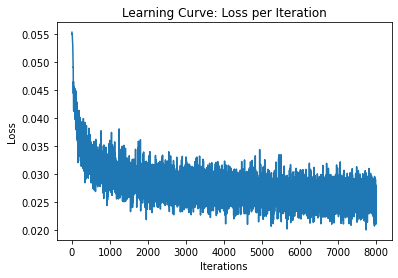
\includegraphics[width=100mm,scale=1]{5b1}\
    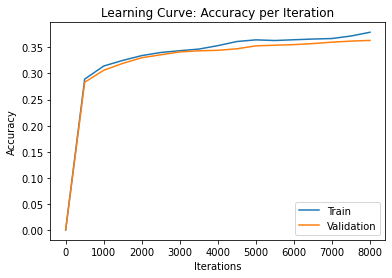
\includegraphics[width=100mm,scale=1]{5b2}\
\end{figure}

Part(c)\\
\begin{python}
def make_prediction_torch(model, sentence):
    """
    Use the model to make a prediction for the next word in the
    sentence using the last 3 words (sentence[:-3]). You may assume
    that len(sentence) >= 3 and that `model` is an instance of
    PyTorchWordEmb. You might find the function torch.argmax helpful.

    This function should return the next word, represented as a string.

    Example call:
    >>> make_prediction_torch(pytorch_model, ['you', 'are', 'a'])
    """
    global vocab_stoi, vocab_itos

    sentence = [word.lower() for word in sentence]
    last = [sentence[-3:]]
    index = convert_words_to_indices(last)
    one_hot = make_onehot(index)
    pred = torch.Tensor(one_hot)
    y = model.forward(pred)
    word_idx = torch.argmax(y)
    return vocab_itos[word_idx.item()]
\end{python}

Part(d)\\
\begin{python}
print(make_prediction_torch(pytorch_model, ['You', 'are', 'a']))
print(make_prediction_torch(pytorch_model, ['few', 'companies', 'show'])) 
print(make_prediction_torch(pytorch_model, ['There', 'are', 'no']))
print(make_prediction_torch(pytorch_model, ['yesterday', 'i', 'was']))
print(make_prediction_torch(pytorch_model, ['the', 'game', 'had'])) 
print(make_prediction_torch(pytorch_model, ['yesterday', 'the', 'federal']))
\end{python}
\begin{python}
good
.
other
nt
been
government
\end{python}
Yes, these predictions do make sense since these are all part of some sentences and look like having the correct relationship with given words.\\
For the 3-grams words, all of the 3-grams words are not appearing next to each other in the training set.\\

Part(e)\\
\begin{python}
print("The test accuracy is", estimate_accuracy_torch(pytorch_model,test4grams))
\end{python}
\begin{python}
The test accuracy is 0.36428347771631353
\end{python}

Question 6. Visualizing Word Embeddings\\

Part(a)\\
\begin{python}
word_emb_weights = list(pytorch_model.word_emb_layer.parameters())[0]
word_emb = word_emb_weights.detach().numpy().T
\end{python}
The shape of the word$\_$emb$\_$weights is (100,250). 100 here represents the emb size and 250
represents the vocab size. This embedding layer is to compute the representation of each word
and we will get the result by multiply the word$\_$emb$\_$weights to the one-hot vector for each
word (which has a shpe 250*1). For each word multiply by woed$\_$emb$\_$weights, we basically do
a matrix multiplication of (100x250) x (250x1) and we will finally get a 100x1 vector and this
vector is the representation vector of that word. If we multiply a (250x250)matrix which
represent all of the one hot vectors for each word. We will finally get a (100x250) matrix which
each column is a word representation vector. But since here we take the transpose, word$\_$emb
has a shape (250,100) which ith row is a 1x100 vector and this vector is the representation of
the ith word in the vocab.In the example vocab$\_$stoi["any"] will get the index of the word "any"
and word$\_$emb[vocab$\_$stoi["any"],:] will take the corresponding row in word$\_$emb matrix.
Which is the vector representation of the word "any".\\

Part(b)\\
\begin{python}
norms = np.linalg.norm(word_emb, axis=1)
word_emb_norm = (word_emb.T / norms).T
similarities = np.matmul(word_emb_norm, word_emb_norm.T)

# Some example distances. The first one should be larger than the second
print(similarities[vocab_stoi['any'], vocab_stoi['many']])
print(similarities[vocab_stoi['any'], vocab_stoi['government']])
\end{python}
\begin{python}
0.393506
-0.06516751
\end{python}
\begin{python}
def closest_words(w):
  similar = similarities[vocab_stoi[w]]
  index = (np.argsort(similar))[::-1]
  print("5 closest words for", w,":")
  for i in range(5):
    print(vocab_itos[index[i]])
  return 
\end{python}
\begin{python}
following_words = ["four", "go","what","should","school","your","yesterday","not"]
for i in following_words:
  closest_words(i)
\end{python}
\begin{python}
5 closest words for four :
four
three
two
five
million
5 closest words for go :
go
back
come
going
get
5 closest words for what :
what
how
who
when
where
5 closest words for should :
should
could
would
might
may
5 closest words for school :
school
states
music
)
department
5 closest words for your :
your
their
our
my
his
5 closest words for yesterday :
yesterday
though
year
today
night
5 closest words for not :
not
nt
never
by
same
\end{python}

Part(c)\\
\begin{python}
import sklearn.manifold
tsne = sklearn.manifold.TSNE()
Y = tsne.fit_transform(word_emb)

plt.figure(figsize=(10, 10))
plt.xlim(Y[:,0].min(), Y[:, 0].max())
plt.ylim(Y[:,1].min(), Y[:, 1].max())
for i, w in enumerate(vocab):
    plt.text(Y[i, 0], Y[i, 1], w)
plt.show()
\end{python}
\begin{figure}[H]
    \centering
    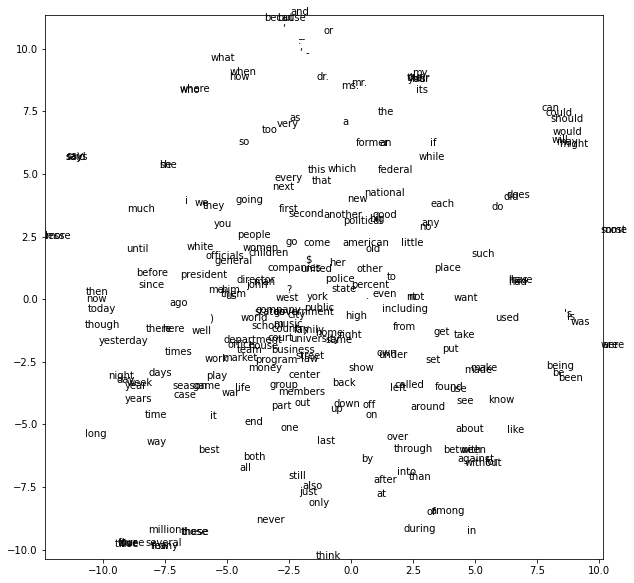
\includegraphics[width=150mm,scale=1]{6c}\
\end{figure}
Cluster 1:\\
many, few,three,two,several\\
---\\
These word in cluster 1 are all able to describe numbers\\
Cluster 2: can,could,will,should,might\\
---\\
These words are all verb and they all can be followed with a personal pronoun\\

Question 7. Work Allocation\\
\begin{python}
#Ming worked on the assignment on Jan 22 - Feb 5, Hongyu worked on the assignment on Jan 22 - Feb 5
# We had meetings on Jan 22, 29 and Feb 4. We also had several short chats during our working time.  
# Ming did Question 1, 3, 5 and Hongyu did question 2, 4, 6
# We checked each other's python code function and discuss the math problems together.
\end{python}
\end{document}